\begin{comment}
\section{JavaScript e a Programação Assíncrona}
A linguagem \textit{JavaScript} teve a sua origem no \textit{browser} \textit{Netscape Navigator} como uma forma de adicionar programas a páginas web.~\cite{elojs} Hoje em dia é usado por grande parte dos \textit{browsers} e tornou possível as aplicações web onde o utilizador pode interagir sem precisar de realizar \textit{refresh} ao fim de cada ação.
Contudo o \textit{Javascript} é bastante liberal no que permite o programador escrever, facilitando a aprendizagem para novos programadores mas tornando a tarefa de resolver e encontrar problemas bem mais difícil visto não apontar aonde estão esses problemas. Ainda assim esta flexibilidade permite uma quantidade de técnicas que não são possíveis em linguagens mais rígidas e que permitem ultrapassar algumas falhas do \textit{Javascript}.~\cite{elojs} 

\subsection{Programação Assíncrona}
Muitos programas em \textit{JavaScript} precisam de por exemplo obter dados através da rede ou a partir do disco. Estes casos são muito mais lentos do que obter os dados a partir de memória para posterior processamento pelo processador. Na realização de tais pedidos o programa em \textit{Javascript} perderia o acesso ao processador, passando este acesso para outro programa que esteja a correr. Só depois de receber o sinal de que o pedido foi efetuado e de ter de novo acesso ao processador é que o programa voltaria a continuar o seu trabalho.

Por forma a evitar perder o acesso do processador em tais casos, e assim realizar trabalho enquanto se espera pela resposta do pedido, o \textit{Javascript} segue um modelo assíncrono. O modelo assíncrono permite que aconteçam várias coisas ao mesmo tempo; quando começa um pedido o programa continua a correr; quando o pedido termina, o programa é informado e tem acesso ao resultado.~\cite{elojs} Para além de não se perder imediatamente o acesso ao processor, o uso de programação assíncrona permite receber e enviar dados de e para múltiplos dispositivos ao mesmo tempo sem complicar a gestão de \textit{threads} e a sincronização necessária em tais casos. Ao usar um modelo assíncrono a expressão de programas que não seguem um modelo de controlo linear é mais fácil enquanto que torna mais difícil aqueles que o seguem.~\cite{elojs}

\subsubsection{\textit{Callbacks}}
Uma abordagem de programação assíncrona é a adição de um argumento extra, uma função \textit{callback}, nas funções que realizam pedidos lentos.~\cite{elojs} Quando o pedido concluir a função \textit{callback} será chamada tendo como argumento o resultado do pedido. Com o uso de callbacks o nível de indentação aumenta com cada pedido assíncrono o que em alguns casos pode tornar o código um pouco difícil de compreender, principalmente nos casos com múltiplos pedidos assíncronos seguidos que têm de ser sequenciais. Para além disso, qualquer função que chame uma função assíncrona tem de ser ela própria assíncrona. Não é recomendado a reestruturação de grandes quantidades de código através de \textit{callbacks} visto ser mais propenso a erros do que retornar apenas um valor.

\begin{lstlisting}[language=javascript, caption=Exemplo de uma \textit{Callback}]
    almocar("comida", function(dentes\_sujos){
        dentes_limpos = lavar_dentes(dentes_sujos)
    })
\end{lstlisting}

\subsubsection{Promessas}
Uma outra abordagem, em vez de passar uma função a ser chamada no futuro, é devolver um objeto que represente este evento futuro, uma promessa. Ou seja, uma promessa é um pedido assíncrono que pode ser concluído no futuro e produzir um valor, tendo a capacidade de notificar qualquer interessado quando o valor estiver disponível.\cite{elojs} O resultado de uma promessa tanto pode já estar pronto ou estar apenas daqui a algum tempo. A principal vantagem das promessas é que simplificam o uso de funções assíncronas visto que não é necessário passar uma função \textit{callback}. Como tal estas funções são similares às restantes mas com uma pequena diferença, o resultado da função pode ainda não estar disponível. 

\begin{lstlisting}[language=javascript, caption=Exemplo de uma Promessa]
    almocar("comida")
        .then(dentes_sujos => dentes_limpos = lavar_dentes(dentes_sujos))
\end{lstlisting}

\subsubsection{Exceções}
Durante a execução de um pedido assíncrono podem ocorrer exceções seja por um erro ou porque por exemplo ocorreu um \textit{time out} do pedido, este último acontece essencialmente quando se realiza pedidos através da rede. Estas exceções precisam de ser tratadas por forma a que o programa que estámos a desenvolver não ``expluda'' deixando de funcionar. Esta tratamento não é simples de se realizar quando se usa \textit{callbacks} enquanto que no caso das promessas basta o uso de um \textit{catch}. No caso das \textit{callbacks} o pedido assíncrono teria de devolver dois valores em vez de um, o primeiro com o erro em caso de insucesso e o segundo com o resultado em caso de sucesso o que obrigaria a função \textit{callback} a verificar se não recebeu uma exceção.

\begin{lstlisting}[language=javascript, caption=Exemplo de uma \textit{Callback} com captura de exceções]
    almocar("comida", function(erro, dentes_sujos){
        if(!erro){
            dentes_limpos = lavar_dentes(dentes_sujos)
        }else{
            console.log("Falta pasta de dentes")
        }
    })
\end{lstlisting}

\begin{lstlisting}[language=javascript, caption=Exemplo de uma Promessa com captura das exceções]
    almocar("comida")
        .then(dentes_sujos => dentes_limpos = lavar_dentes(dentes_sujos))
        .catch(erro => console.log("Falta pasta de dentes"))
\end{lstlisting}

\subsubsection{Funções \textit{async}}
Dentro de funções \textit{async} é possível escrever código pseudo-síncrono por forma a descrever código assíncrono com recurso ao \textit{await} que espera pela conclusão de uma promessa antes de avançar com a execução do resto da função, ficando o código com um aspeto semelhante ao síncrono. As funções \textit{async} retornam implicitamente uma promessa e enquanto estão à espera duma promessa (\textit{await}) ficam congeladas. Serão resumidas mais tarde quando a promessa estiver concluída.

\begin{lstlisting}[language=javascript, caption=Exemplo de uma função \textit{async}]
    async function almoco(){
        try{
            dentes_sujos = await almocar("comida")
            dentes_limpos = lavar_dentes(dentes_sujos)
        }catch(erro){
            console.log("Falta pasta de dentes")
        }
        return "Almocei!"
    }
\end{lstlisting}

\section{Node.js}
\textit{Node.js} é um ambiente de execução que permite usar \textit{JavaScript} fora do contexto de um \textit{browser} permitindo construir desde ferramentas de linha de comandos até servidores \acrshort{http}. Foi originalmente desenhado de forma a ter o papel de nodo numa rede. O \textit{JavaScript} não tem embutido a capacidade de entrada e saída de dados sendo suprimida esta necessidade com o uso do \textit{Node.js}.

Quando instalado num sistema, o \textit{Node.js} permite executar ficheiros \textit{JavaScript} através do comando \texttt{node}. Se este comando for executado sem indicar um ficheiro apresenta uma consola interativa onde se pode introduzir código \textit{JavaScript}, executá-lo e obter o resultado.

Através do \acrshort{npm}, mais precisamente do comando \texttt{npm}, é possível instalar, no nosso projeto pessoal, os módulos \textit{JavaScript} disponíveis no repositório \textit{online}. Caso exista um ficheiro \textit{package.json} no projeto é mantido neste os módulos já instalados e as suas versões bem como meta informação do projeto.

Em \textit{Node.js} estão disponíveis os \textit{bindings} globais \texttt{process} e \texttt{console} que permitem inspecionar e manipular o programa atual. Para além destes, também estão diponíveis os \textit{bindings} padrão do \textit{JavaScript} exceto aqueles relacionados com funcionalidades do \textit{browser}, como o \texttt{document}.

O \textit{Node.js} tem algums módulos embutidos, entre os quais o módulo \texttt{fs} (\textit{file system}) que exporta funções que permitem trabalhar com ficheiros e directorias. Tem também o módulo \texttt{http} que exporta funções que permitem correr servidores \acrshort{http} ou fazer pedidos \acrshort{http}.

Todo o input e output no \textit{Node.js} é realizado de forma assíncrona a menos que se use uma variante síncrona de uma determinada função.~\cite{elojs}
\end{comment}

\section{Estado da Arte do \acrshort{clav}}

Quando esta dissertação teve início o projeto \acrshort{clav} já tinha cerca de 2 anos de desenvolvimento. Assim nesta secção será apresentado o estado da arte do \acrshort{clav} quando esta dissertação iniciou aprofundando principalmente os pontos mais importantes sobre o tema desta dissertação.

\subsection{Estrutura}
O \acrshort{clav} está dividido em duas partes:
\begin{itemize}
    \item interface (\textit{front-end}) presente em \url{http://clav.dglab.gov.pt}
    \item \acrshort{api} de dados (\textit{back-end} que inclui também duas bases de dados, \textit{GraphDB} e \textit{MongoDB}) presente em \url{http://clav-api.dglab.gov.pt}.
\end{itemize}

Cada parte encontra-se numa máquina diferente.

Através da figura~\ref{fig:clav_struct} é possível ver o possível fluxo tanto de um utilizador a aceder à interface como a de um utilizador a aceder diretamente à \acrshort{api} de dados. No primeiro caso, quando um utilizador acede o servidor da interface do \acrshort{clav} é descarregado para o lado do utilizador o ficheiro \acrshort{html} (\textit{index}) e os vários ficheiros \textit{JavaScript}, \acrshort{css} e \textit{assets} (como imagens, \acrshort{pdf}s, etc) quando necessários. O servidor da interface é nada mais que um servidor \textit{web} com recurso ao \textit{Nginx} que hospeda estes ficheiros, os quais representam a interface construída com o \textit{Vue} e o \textit{Vuetify}. Como tal o código apresenta-se todo do lado do utilizador e os pedidos à \acrshort{api} serão feitos do computador do utilizador para o servidor da \acrshort{api} de dados e não do servidor da interface para o servidor da \acrshort{api} de dados. Ou seja, o fluxo de cada um desses pedidos será igual ao fluxo no caso em que se acede diretamente a \acrshort{api} sem uso de qualquer interface.

\begin{figure}[H]
    \begin{center}
        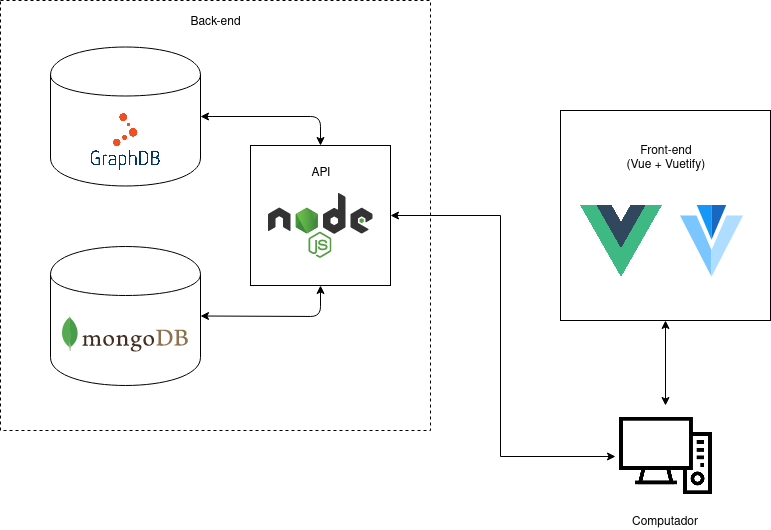
\includegraphics[width=0.7\textwidth]{img/clav_struct.png}
    \end{center}
    \caption{Estrutura do \acrshort{clav} incluíndo a interação de um utilizador com a mesma}\label{fig:clav_struct}
\end{figure}

\subsection{Formas de autenticação}\label{sec:autenticacao}
A \acrshort{api} de dados e a interface estavam inicialmente ``juntas'' (aplicação monolítica) onde as rotas eram protegidas contudo, com a separação da aplicação em duas partes, ambas partes deixaram de estar protegidas. Devido à plataforma já ter estado protegida esta já possui duas formas de autenticação, através de chaves \acrshort{api} ou através de utilizadores registados. Ou seja, tanto o registo de utilizadores e de chaves API já se encontra implementado bem como o \textit{login} de utilizadores.

As chaves \acrshort{api} existem por forma a dar acesso a certas rotas da \acrshort{api} a aplicações que interajam com a mesma (por exemplo sistemas de informação) sem a necessidade de interação humana.

Já os utilizadores possuem múltiplos níveis de acesso sendo que consoante o seu nível podem ou não aceder a uma rota da interface ou da \acrshort{api}. Os utilizadores podem autenticarem-se através de \textit{email} e \textit{password} ou com recurso ao \acrfull{cc} através do Autenticação.gov, este último apenas disponível através da interface do \acrshort{clav}.

A hierarquia dos níveis de acesso, do nível que permite menor para o maior acesso, é a seguinte:
\begin{itemize}
    \item Nível 0: Chaves API
    \item Nível 1: Representante Entidade
    \item Nível 2: Utilizador Simples
    \item Nível 3: Utilizador Avançado
    \item Nível 3.5: Utilizador Validador (AD)
    \item Nível 4: Utilizador Validador
    \item Nível 5: Utilizador Decisor
    \item Nível 6: Administrador de Perfil Funcional
    \item Nível 7: Administrador de Perfil Tecnológico
\end{itemize}

As chaves \acrshort{api} poderão aceder a algumas rotas com método \texttt{GET}.
Já os utilizadores poderão realizar todos os pedidos que as chaves \acrshort{api} podem realizar mas quanto maior o seu nível de acesso mais rotas poderão aceder.

A proteção da \acrshort{api} terá de ter esta hierarquia em conta.

\subsubsection{Registo}

Como já referido tanto o registo de chaves \acrshort{api} como de utilizadores já se encontra implementado.

Para o registo de uma chave \acrshort{api} é necessário providenciar um nome, um email e a entidade a que pertence. Após o registo da chave a informação desta chave \acrshort{api} é mantida numa base de dados \textit{MongoDB}.

Um utilizador pode se registar através de \texttt{email + password} ou através do Autenticação.gov. No primeiro caso, ao se registar necessita obviamente de indicar o seu email, a \textit{password}, o seu nome, a entidade a que pertence e o nível de acesso que pretende. Já no caso do Autenticação.gov para o registo do utilizador é necessário todos os campos anteriores exceto a \textit{password} (pode ser depois definida), sendo também necessário o campo \acrfull{nic} do utilizador. Caso o registo seja efetuado com recurso à interface do Autenticação.gov apenas será necessário indicar o email, a entidade a que pertence e o nível de acesso que pretende visto que os restantes campos são fornecidos pela Autenticação.gov quando o utilizador se autentica e autoriza nesta a partilha dessa informação com a plataforma do \acrshort{clav}.
A \textit{password} é armazenada não na sua forma literal mas sim a sua \textit{hash} ao aplicar a função criptográfica \texttt{bcrypt}. A utilização de funções de \textit{hash} criptográficas ao armazenar \textit{passwords} impede que as \textit{passwords} originais se saibam caso a base de dados seja comprometida. Para além disso, como o \texttt{bcrypt} combina um valor aleatório (\texttt{salt}) com a \textit{password} do utilizador, é impossível pré-computar a \textit{password} que deu origem ao \textit{hash} sem saber o \texttt{salt}\footnote{Para mais informação veja \textit{rainbow table attack}}.

Durante esta tese com a proteção da \acrshort{api} ficará apenas possível o registo de utilizadores através de utilizadores que já estejam registados e possuam um nível de acesso suficiente para registar utilizadores. Estes utilizadores registados e autorizados pertencem à entidade \acrshort{dglab}. Portanto por forma a utilizadores representantes de outras entidades se registarem na plataforma terão de:~\cite{clavwebpage}
\begin{itemize}
    \item Preencher o formulário disponibilizado para o efeito, para cada representante designado pela entidade;
    \item O formulário deverá ser assinado por um dirigente superior da Entidade e autenticado com assinatura digital, se o envio for feito por via eletrónica (NB\@: não serão aceites assinaturas do formulário por dirigentes intermédios). Esta autorização autenticada pelo dirigente superior é o equivalente a uma delegação de competências, uma vez que o representante da entidade passa a ter capacidade para, em nome da entidade, submeter autos de eliminação, propostas de tabelas de seleção e novas classes para a Lista Consolidada;
    \item O formulário deverá ser remetido à \acrshort{dglab} por via postal ou eletrónica, respetivamente, para:
    \begin{itemize}
        \item \acrshort{dglab}, Edifício da Torre do Tombo, Alameda da Universidade, 1649--010 Lisboa (formulário assinado manualmente) ou
        \item clav@dglab.gov.pt (formulário com assinatura digital).
    \end{itemize}
    \item Após receção do formulário, a \acrshort{dglab} efetuará o(s) respetivo(s) registo(s) até 48 horas úteis;
    \item Findo esse prazo, o utilizador poderá aceder à plataforma, selecionando a opção ``Autenticação'';
    \item A autenticação, no primeiro acesso, deve ser efetuada com o \acrlong{cc}.
\end{itemize}

\subsubsection{\textit{Login}}

O \textit{login} apenas está presente para o caso dos utilizadores visto que assim que uma chave \acrshort{api} é registada é enviado por email um \acrshort{jwt} com a duração de 30 dias a ser usado nos pedidos a realizar à \acrshort{api}. O utilizador poderá ao fim dos 30 dias renovar a sua chave \acrshort{api}, onde é gerado um novo \acrshort{jwt}.

Portanto do lado dos utilizadores é possível como já referido realizar o \textit{login} de duas formas através de uma estratégia local ou através do Autenticação.gov.

A estratégia local (\texttt{email + password}) é conseguida através do uso do \textit{middleware} \textit{Passport}.
O \textit{Passport} é um middleware de autenticação para \textit{Node.js} que tem como objetivo autenticar pedidos.~\cite{passport} Tem como única preocupação a autenticação delegando qualquer outra funcionalidade para a aplicação que a usa. Este \textit{middleware} possui muitas estratégias de autenticação entre as quais a local (\texttt{email/username + password}), \acrshort{jwt}, \textit{OAuth}\footnote{Protocolo \textit{open-source} com o objetivo de permitir a autenticação simples, segura e padrão entre aplicações móveis, \textit{web} e \textit{desktop}}, \textit{Facebook} ou \textit{Twitter}. Cada estratégia está num módulo independente. Assim as aplicações que usam o \textit{Passport} não terão um peso adicional devido a estratégias que nem sequer usam.

No caso do \textit{login} através do Autenticação.gov, o utilizador tem de se autenticar na interface do Autenticação.gov (a partir do botão disponível na área de autenticação da interface do \acrshort{clav}). O fluxo do \textit{login} neste caso é: 

\begin{figure}[H]
    \begin{center}
        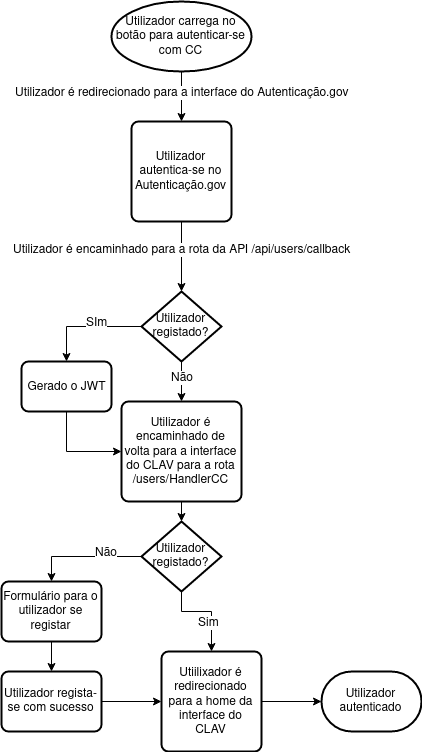
\includegraphics[width=0.5\textwidth]{img/authgov.png}
    \end{center}
    \caption{Fluxo do \textit{login} de um utilizador através do Autenticação.gov}\label{fig:authgov}
\end{figure}

No \textit{login} do utilizador é gerado um \acrshort{jwt} com a duração de 8 horas que deve ser usado nos pedidos a realizar à \acrshort{api}. No fim das 8 horas o utilizador necessita de se autenticar de novo.

%TODO
%\subsection{Lista Consolidada}

%TODO
%\subsection{Tabelas de Seleção}

%TODO
%\subsection{Cache e Fecho Transitivo}

%TODO
%\section{\acrshort{rest}}
%~\cite{restws}

%TODO
%\section{express}
%\cite{wdmongo}
%procurar "semelhantes" para cada um

\section{\acrfull{jwt}}
O \acrshort{jwt} é um \textit{open standard}\footnote{Mais informação em \url{https://tools.ietf.org/html/rfc7519}} que define uma forma compacta e independente de transmitir com segurança informação entre partes com um objeto \acrshort{json}.~\cite{jwtio} O \acrshort{jwt} pode ser assinado digitalmente (\acrshort{jws}), encriptado (\acrshort{jwe}), assinado e depois encriptado (\acrshort{jws} encriptado, ou seja, um \acrshort{jwe}, ordem recomendada\footnote{Mais informação em \url{https://tools.ietf.org/html/rfc7519\#section-11.2}}) ou encriptado e depois assinado (\acrshort{jwe} assinado, ou seja, um \acrshort{jws}).

Caso seja assinado digitalmente é possível verificar a integridade da informação mas não é garantida a sua privacidade contudo podemos confiar na informação do \acrshort{jwt}. A assinatura pode ser efetuada através de um segredo usando por exemplo o algoritmo \acrshort{hmac} ou através de pares de chaves pública/privada usando por exemplo o algoritmo \acrshort{rsa}. No caso de se usar pares de chaves pública/privada a assinatura também garante que a parte envolvida que tem a chave privada é aquela que assinou o \acrshort{jwt}.

Por outro lado, os \acrshort{jwt}s podem ser encriptados garantindo a privacidade destes, escondendo a informação das partes não envolvidas. Nesta secção apenas se falará sobre \acrshort{jwt}s e \acrshort{jws}s (\acrshort{jwt} assinado). Se pretender saber mais sobre \acrshort{jwe}s pode ler o capítulo 5 do livro \textit{The JWT Handbook} por \textit{Sebastián E. Peyrott}.

Sendo assim em que casos é útil o uso de \acrshort{jwt}s? Dois dos casos são os seguintes:
\begin{itemize}
    \item Autorização: Este será o caso para o qual o \acrshort{jwt} será usado na \acrshort{clav}. Quando o utilizador realiza o \textit{login} gera-se um \acrshort{jwt} por forma a que os restantes pedidos desse utilizador sejam realizados com esse \acrshort{jwt} (\textit{Single Sign On}). O uso de \acrshort{jwt}s para estes casos permitem um \textit{overhead} pequeno e a flexibilidade de serem usados em diferentes domínios.
    \item Troca de informação: No caso de troca de informação entre duas partes os \acrshort{jwt}s assinados são de bastante utilidade visto que permitem verificar se o conteúdo não foi violado e, no caso de se usar pares de chaves pública/privada para assinar, permitem ter a certeza que o remetente é quem diz ser.
\end{itemize}

\subsection{Estrutura do \acrshort{jwt}}

Os \acrshort{jwt}s são construídos a partir de três elementos, o \textit{header} (objeto \acrshort{json} também conhecido por \acrshort{jose} \textit{header}), o \textit{payload} (objeto \acrshort{json}) e os dados de assinatura/encriptação (depende do algoritmo usado). Estes elementos são depois codificados em representações compactas (\texttt{Base64 URL-safe}\footnote{Variante da codificação \texttt{Base64} onde a codificação gerada é segura para ser usada em \textit{URL}s. Basicamente para a codificação \texttt{Base64} gerada substitui os caracteres '+' e '/' pelos caracteres '-' e '\_' respetivamente. Além disso, remove o caracter de \textit{padding} e proibe separadores de linha}). As codificações \texttt{Base64 URL-safe} de cada elemento são depois concatenadas através de pontos dando origem a uma representação final compacta do \acrshort{jwt} (\textit{JWS/JWE Compact Serialization}). Na secção~\ref{sec:criacaojwt} está presente dois diagramas referentes à construção de dois \acrshort{jwt}s sendo um deles assinado.

\begin{figure}[H]
    \centering
    \textbf{\textcolor{red}{eyJhbGciOiJIUzI1NiIsInR5cCI6IkpXVCJ9}.
        \textcolor{purple}{eyJuYW1lIjoiSm9zw6kgTWFydGlucyIsIm51bSI6ImE3ODgyMSJ9}.
        \textcolor{cyan}{tRPSYVsFI-nziRPuAjdGZLN2tUez5MtLML\_aAnPplgM}
    }
    \caption{Exemplo de representação compacta de \acrshort{jwt} (quebra de linhas por forma a melhorar leitura)}\label{fig:exemjwt}
\end{figure}

De seguida vamos aprofundar cada elemento referido:
\begin{itemize}
    \item[\textbf{\textit{Header}:}]

    O cabeçalho (a vermelho na figura~\ref{fig:exemjwt}) consiste nos seguintes atributos:
    \begin{itemize}
        \item O atributo obrigatório (único campo obrigatório para o caso de um \acrshort{jwt} não encriptado) \texttt{alg} (algorítmo) onde é indicado que algoritmo é usado para assinar e/ou desencriptar. O seu valor pode ser por exemplo HS256 (\acrshort{hmac} com o auxilio do SHA-256\footnote{Função pertencente ao conjunto de funções \textit{hash} criptográficas \acrfull{sha2} desenhadas pela \acrshort{nsa}}) ou \acrshort{rsa}.
        \item O atributo opcional \texttt{typ} (tipo do \textit{token}) em que o seu valor é ``JWT''. Serve apenas para distinguir os \acrshort{jwt}s de outros objetos que têm um \acrshort{jose} \textit{header}.
        \item O atributo opcional \texttt{cty} (tipo do conteúdo (\textit{payload})). Se o \textit{payload} conter atributos arbitrários este atributo não deve ser colocado. Caso o \textit{payload} for um \acrshort{jwt}\footnote{\acrshort{jwt} aninhado (\textit{nested \acrshort{jwt}})} então este atributo deve ter o valor de ``JWT''.
    \end{itemize}

    O cabeçalho é de grande importância visto que permite saber se o \acrshort{jwt} é assinado ou encriptado e de que forma o resto do \acrshort{jwt} deve ser interpretado.

    \begin{lstlisting}[language=json, caption=\textit{Header} usado para construir o \acrshort{jwt} da figura~\ref{fig:exemjwt}]
    {
        "alg": "HS256",
        "typ": "JWT"
    }
    \end{lstlisting}

    \item [\textbf{\textit{Payload}:}] O \textit{payload} (a roxo na figura~\ref{fig:exemjwt}) contém a informação/dados que pretendemos transmitir com o \acrshort{jwt}. Não há atributos obrigatórios contudo existem certos atributos que têm um significado definido (atributos registados).

    Existem 7 atributos registados (\textit{registered claims}):~\cite{jwthandbook}
    \begin{itemize}
        \item \texttt{iss} (\textit{issuer}): Identificador único (\textit{case-sensitive string}) que identifica unicamente quem emitiu o \acrshort{jwt}. A sua interpretação é específica a cada aplicação visto que não há uma autoridade central que gere os emissores.
        \item \texttt{sub} (\textit{subject}): Identificador único (\textit{case-sensitive string}) que identifica unicamente de quem é a informação que o \acrshort{jwt} transporta. Este atributo deve ser único no contexto do emissor, ou se tal não for possível, globalmente único. O tratamento do atributo é específico a cada aplicação. 
        \item \texttt{aud} (\textit{audience}): Identificador único (\textit{case-sensitive string}) ou \textit{array} destes identificadores únicos que identificam unicamente os destinatários pretendidos do \acrshort{jwt}. Ou seja, quem lê o \acrshort{jwt} se não estiver no atributo \texttt{aud} não deve considerar os dados contidos no \acrshort{jwt}. O tratamento deste atributo também é específico a cada aplicação. 
        \item \texttt{exp} (\textit{expiration (time)}): Um número inteiro que representa uma data e hora específica no formato \textit{seconds since epoch} definido pela \acrshort{posix}\footnote{Mais informação em \url{https://pubs.opengroup.org/onlinepubs/9699919799/basedefs/V1\_chap04.html\#tag\_04\_16}}, a partir da qual o \acrshort{jwt} é considerado inválido (expira).
        \item \texttt{nbf} (\textit{not before (time)}): Representa o inverso do atributo \texttt{exp} visto que é um número inteiro que representa uma data e hora específica no mesmo formato do atributo \texttt{exp}, mas que a partir da qual o \acrshort{jwt} é considerado válido.
        \item \texttt{iat} (\textit{issued at (time)}): Um número inteiro que representa uma data e hora especifica no mesmo formato dos atributos \texttt{exp} e \texttt{nbf} na qual o \acrshort{jwt} foi emitido.
        \item \texttt{jti} (\textit{\acrshort{jwt} ID}): Identificador único (\textit{string}) do \acrshort{jwt} que permite distinguir \acrshort{jwt}s com conteúdo semelhante. A implementação tem de garantir a unicidade deste identificador.
    \end{itemize}

    Estes atributos registados têm todos 3 caracteres visto que um dos requisitos do \acrshort{jwt} é ser o mais pequeno/compacto possível.

    Existem depois mais dois tipos de atributos, públicos e privados. Os atributos públicos podem ser definidos à vontade pelos utilizadores de \acrshort{jwt}s mas têm de ser registados em \textit{IANA JSON Web Token Claims registry} ou definidos por um espaço de nomes resistente a colisões de forma a evitar a colisão de atributos. Já os atributos privados são aqueles que não são nem registados nem públicos e podem ser definidos à vontade pelos utilizadores de \acrshort{jwt}s. Os dois atributos usados no exemplo~\ref{exem:pay} (\texttt{name} e \texttt{num}) são atributos privados.

    \begin{lstlisting}[language=json, caption=\textit{Payload} usado para construir o \acrshort{jwt} da figura~\ref{fig:exemjwt}, label=exem:pay]
    {
        "name": "José Martins",
        "num": "a78821"
    }
    \end{lstlisting}

\item [\textbf{\textit{Signature}:}] A assinatura (a azul da figura~\ref{fig:exemjwt}) é criada ao usar o algoritmo indicado na \textit{header} no atributo \texttt{alg} tendo como um dos argumentos os elementos codificados da \textit{header} e do \textit{payload} juntos por um ponto e como outro argumento um segredo. O resultado do algoritmo é depois codificado em \texttt{Base64 URL-safe}. Esta assinatura no caso dos \acrshort{jws}s é usada para verificar a integridade do \acrshort{jwt} e caso seja assinado com uma chave privada permite também verificar se o remetente é quem diz ser. No caso de o atributo \texttt{alg} for \texttt{none} a assinatura é uma \texttt{string} vazia.

    \begin{lstlisting}[language=javascript, caption=\textit{Signature} usado para construir o \acrshort{jwt} da figura~\ref{fig:exemjwt}]
    HMACSHA256(
        base64UrlEncode(header) + "." +
        base64UrlEncode(payload),
        segredo1.-uminho!clav
    )
    \end{lstlisting}
\end{itemize}

\subsection{Criação de \acrshort{jwt}/\acrshort{jws}}\label{sec:criacaojwt}

Na figura~\ref{fig:buildJWT} é apresentada a construção de um \acrshort{jwt} em que o atributo \texttt{alg} (algorítmo) tem o seu valor igual a \texttt{none}, ou seja, o \acrshort{jwt} não é assinado nem encriptado.

\begin{figure}[H]
    \begin{center}
        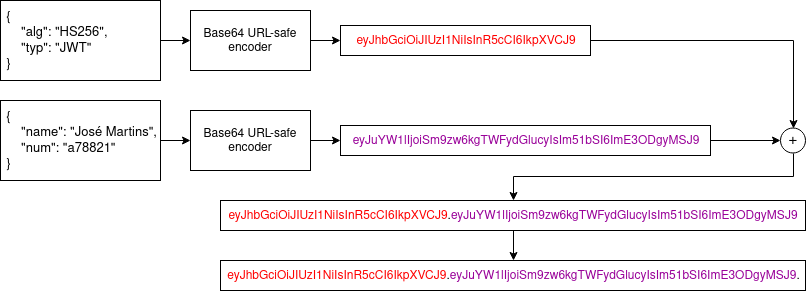
\includegraphics[width=1\textwidth]{img/buildJWT.png}
    \end{center}
    \caption{Criação de um \acrshort{jwt}}\label{fig:buildJWT}
\end{figure}

Já na figura~\ref{fig:buildJWS} é demonstrada a construção de um \acrshort{jwt} assinado, ou seja, um \acrshort{jws}.

\begin{figure}[H]
    \begin{center}
        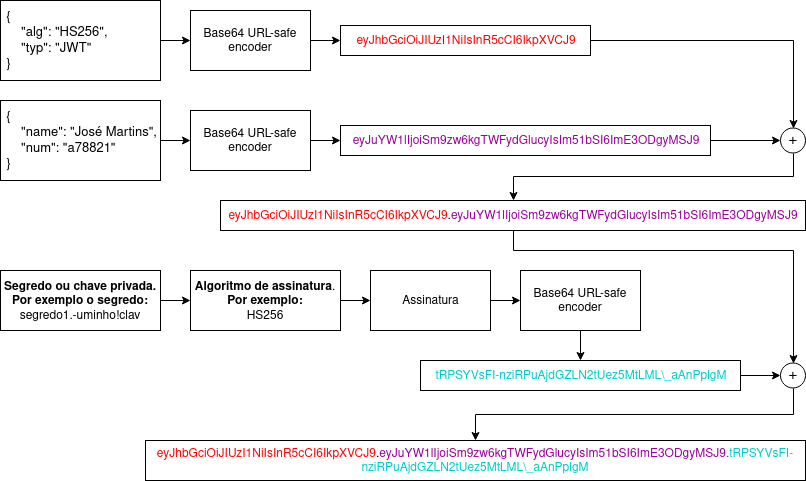
\includegraphics[width=1\textwidth]{img/buildJWS.png}
    \end{center}
    \caption{Criação de um \acrshort{jws}}\label{fig:buildJWS}
\end{figure}

\subsection{Alternativas ao \acrshort{jwt}}

Algumas alternativas ao \acrshort{jwt} passam pelo uso de \acrfull{swt} ou \acrfull{saml}. Se compararmos o \acrshort{jwt} ao \acrshort{saml}, o \acrshort{json} é menos verboso que o \acrshort{xml} e mesmo quando codificado o seu tamanho é menor. 

De um ponto de vista de segurança o \acrshort{swt} apenas pode ser assinado simetricamente por um segredo partilhado usando o algoritmo \acrshort{hmac}. Já o \acrshort{jwt} e o \acrshort{saml} podem usar pares de chaves pública/privada para assinar. Contudo assinar \acrshort{xml} com \textit{\acrshort{xml} Digital Signature} sem introduzir buracos de segurança é mais dificil quando comparado com a simplicidade de assinar \acrshort{json}.~\cite{jwtio}

Houve contudo algumas bibliotecas de \acrshort{jwt} com vulnerabilidades devido ao atributo \texttt{alg} da \textit{header} do \acrshort{jwt}. Havia duas situações de vulnerabilidade:
\begin{itemize}
    \item As bibliotecas ao fazer a verificação (recebe um \acrshort{jwt} e um segredo/chave pública como argumentos) de um \acrshort{jwt} com \texttt{alg} igual a \texttt{none} assumiam logo que o \acrshort{jwt} era válido mesmo que o segredo/chave pública fosse diferente de vazio. Ou seja, com a simples alteração do atributo \texttt{alg} e com a remoção da \textit{signature} podia-se alterar o \textit{payload} do \acrshort{jwt} que o servidor iria continuar a considerar que a integridade do \acrshort{jwt} não foi colocada em causa mesmo que os \acrshort{jwt}s gerados pelo servidor tivessem sido com um algoritmo e com recurso a um segredo/chave privada.
    \item As bibliotecas ao fazer a verificação seja um algoritmo simétrico ou assimétrico apenas tinham como parâmetros o \acrshort{jwt} e o segredo/chave pública. Isto gera uma segunda vulnerabilidade, se o servidor estiver à espera de um \acrshort{jwt} assinado com pares de chaves pública/privada mas recebe um \acrshort{jwt} assinado com \acrshort{hmac} vai assumir que a chave pública é o segredo a usar no algoritmo \acrshort{hmac}. Ou seja, se se criar um \acrshort{jwt} com o atributo \texttt{alg} igual a \acrshort{hmac} e a assinatura for gerada usando o algoritmo \acrshort{hmac} com o segredo a ser a chave pública, podemos alterar o \textit{payload} (antes de assinar) que o servidor vai considerar que o \acrshort{jwt} não foi maliciosamente alterado.
\end{itemize}

Portanto a flexibilidade de algoritmos dada pelo \acrshort{jwt} coloca em causa a segurança pelo que da parte das bibliotecas o atributo \texttt{alg} não deve ser considerado~\cite{jwtvuln} bem como deve ser \textit{deprecated} e deixar de ser incluído nos \acrshort{jwt}s\footnote{Ver \url{https://gist.github.com/paragonie-scott/c88290347c2589b0cd38d8bb6ac27c03}}. 

A biblioteca que será usada na \acrshort{clav}, \texttt{jsonwebtoken}, já endereçou estes problemas\footnote{Ver \url{https://github.com/auth0/node-jsonwebtoken/commit/1bb584bc382295eeb7ee8c4452a673a77a68b687}} pelo que estas vulnerabilidades não estarão presentes na \acrshort{clav}.

Por outro os \textit{parsers} de \acrshort{json} são mais comuns em grande parte das linguagens de programação visto que os \acrshort{json}s mapeiam diretamentepara objetos ao contrário do \acrshort{xml} que não tem um mapeamento natural de documento para objeto.~\cite{jwtio} Portanto isto torna mais fácil trabalhar com \acrshort{jwt} do que com \acrshort{saml}.

Já quando comparamos os \acrshort{jwt} a \textit{cookie sessions}, o \acrshort{jwt} tem a vantagem de as sessões puderem ser \textit{stateless} enquanto que as \textit{cookies} são \textit{statefull}. Contudo, ser \textit{stateless} não permite por exemplo que a qualquer altura se possa revogar um \acrshort{jwt}. Para endereçar esse problema é necessário, por exemplo, guardar (\textit{statefull}) os \acrshort{jwt}s numa base de dados associando cada \acrshort{jwt} ao identificador único de quem é a informação contida no \acrshort{jwt} (o uso de uma \textit{whitelist}). Assim para revogar um \acrshort{jwt} bastaria removê-lo da base de dados.

%TODO: referencia para API gateways
Outra alternativa ao \acrshort{jwt} seria \textit{sessionIDs}. As \textit{sessionIDs} são \textit{strings} longas, únicas e aleatórias. É possível revogar um \textit{sessionID}, ao contrário do \acrshort{jwt}, bastando para isso remover o \textit{sessionID} da base de dados. Mais à frente na secção~\ref{} veremos outra possível alternativa com recurso a \acrshort{api} \textit{gateways} em que uma possível abordagem é dentro da \acrshort{api} \textit{gateway} ser através de \acrshort{jwt}s, fora ser usado \textit{sessionIDs} e na ``entrada'' da \acrshort{api} \textit{gateway} ter uma base de dados que associa os \textit{sessionsIDs} aos \acrshort{jwt}s.

Por fim, uma outra alternativa bastante semelhante ao \acrshort{jwt} é \textit{Branca}. \textit{Branca} usa o algoritmo simétrico \textit{\acrshort{ietf} XChaCha20-Poly1305 \acrshort{aead}} que permite criar \textit{tokens} encriptados e que garantam integridade. Tem também uma região de \textit{payload} como \acrshort{jwt} com a única diferença é que este \textit{payload} não tem um estrutura definida. Não necessita da \textit{header} visto que o algoritmo usado não varia. Em vez de usar codificação em \texttt{Base64 URL-safe} usa \texttt{Base62} que também é \textit{URL-safe}. Para além disso o \textit{token} gerado é geralmente de menor dimensão do que o gerado pelo \acrshort{jwt} sendo como tal mais compacto que o \acrshort{jwt}.~\cite{branca} Visto que o \textit{Branca} encripta e garante integridade de uma forma mais simples que o \acrshort{jwt} permite (para isso era necessário recorrer a um \acrshort{jwe} que tem no seu \textit{payload} um \acrshort{jws}), sendo como tal propenso a menos erros de programação. Contudo, o \textit{Branca} ainda não é muito conhecido nem um \textit{standard} da indústria, ao contrário do \acrshort{jwt}, mas não deixa de ser algo a ter em conta para o futuro. 

\section{Autorização de pedidos à \acrshort{api}}

Quanto à forma como os pedidos serão feitos à \acrshort{api} poderão ser feitos de duas formas, através da \textit{header} \acrshort{http} \textit{Authorization} ou através da \textit{query string} do pedido em um dos seguintes campos:
\begin{itemize}[leftmargin=3cm]
    \item[\textbf{\texttt{token}}] caso seja o \texttt{token} de um utilizador:\newline
        \verb|http://example.com/path/page?token=<token>|
    \item[\textbf{\texttt{apikey}}] caso seja uma Chave \acrshort{api}:\newline
        \verb|http://example.com/path/page?apikey=<Chave API>|
\end{itemize}

Na \textit{header} \textit{Authorization} irá se usar o esquema de autenticação \textit{Bearer}\footnote{Mais informação em \url{https://tools.ietf.org/html/rfc6750}} com umas pequenas alterações. Portanto o conteúdo da \textit{header} \textit{Authorization}:
\begin{itemize}[leftmargin=2cm]
    \item Caso seja o \texttt{token} de um utilizador:\newline
        \verb|token <token>|
    \item Caso seja uma Chave \acrshort{api}:\newline
        \verb|apikey <Chave API>|
\end{itemize}
ao invés do esquema de autenticação predefenido do \textit{Bearer}: \verb|Bearer <token/Chave API>|

Convém referir que a Chave \acrshort{api} é também um \textit{token}. A divisão entre utilizadores e chaves \acrshort{api} permite uma mais fácil gestão dos \textit{tokens} recebidos pela \acrshort{api} bem como usar duas formas diferentes de os gerar/verificar com o possível benefício de melhorar a segurança da \acrshort{api}.

Os \textit{token}s gerados pela \acrshort{api} serão \acrshort{jwt}s. Contudo poderiam ser outro tipo de \textit{tokens} (por exemplo uma \textit{string} aleatória e única) que o processo de envio dos \textit{tokens} para a \acrshort{api} manter-se-ia igual. 

Após descrito como poderão ser feitos os pedidos à \acrshort{api}, irá ser apresentado possíveis fluxos de interação entre utilizadores (\textit{browser}, \textit{app}, etc) e o servidor da \acrshort{api}. 

O fluxo de autenticação de um utilizador na \acrshort{api} a ser implementado será o seguinte:
\begin{figure}[H]
    \begin{center}
        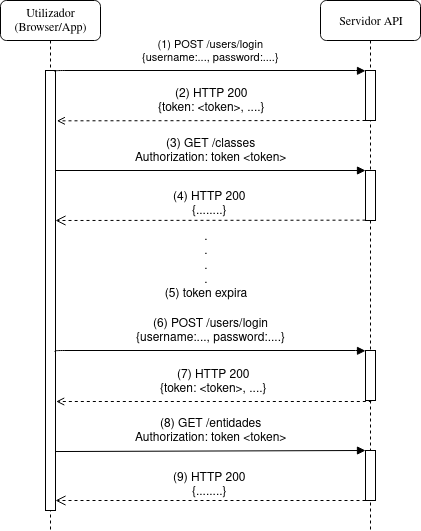
\includegraphics[width=0.5\textwidth]{img/userAuth.png}
    \end{center}
    \caption{Fluxo de autenticação e posteriores pedidos de um utilizador}\label{fig:userAuth}
\end{figure}

\begin{enumerate}
    \item Utilizador autentica-se ao providenciar o seu \textit{email} e a sua \textit{password}
    \item Caso o utilizador se autentique com sucesso é devolvido um \textit{token} que deve ser usado nos restantes pedidos até expirar
    \item Utilizador realiza um pedido para obter as classes, colocando o token na \textit{header} \textit{Authorization}
    \item Caso o \textit{token} enviado seja válido e não tenha expirado são devolvidas as classes
    \item \textit{Token} expirou após o tempo definido
    \item Utilizador realiza uma nova autenticação por forma a obter um novo \textit{token}
    \item Caso o utilizador se autentique com sucesso é devolvido um \textit{token} que deve ser usado nos restantes pedidos até expirar
    \item Utilizador realiza um pedido para obter as entidades, colocando o token na \textit{header} \textit{Authorization}
    \item Caso o \textit{token} enviado seja válido e não tenha expirado são devolvidas as entidades
\end{enumerate}

O fluxo de autenticação e renovação de uma Chave \acrshort{api} na \acrshort{api} a ser implementado será o seguinte:
\begin{figure}[H]
    \begin{center}
        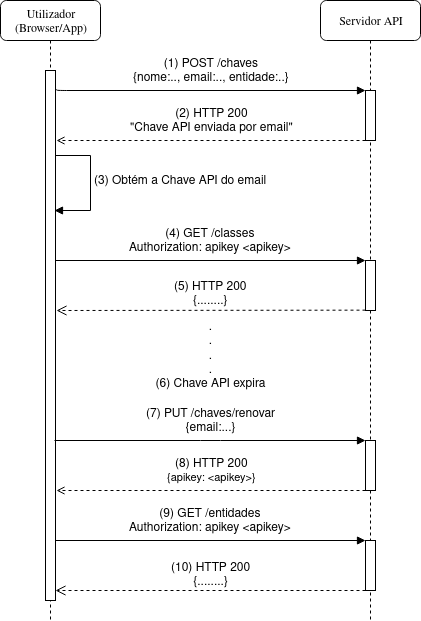
\includegraphics[width=0.5\textwidth]{img/chaveAuth.png}
    \end{center}
    \caption{Fluxo de autenticação e posteriores pedidos de uma chave \acrshort{api}}\label{fig:chaveAuth}
\end{figure}

\begin{enumerate}
    \item Utilizador cria uma chave \acrshort{api} ao providenciar o nome, email e entidade
    \item A Chave \acrshort{api} é enviada para o email fornecido pelo utilizador com o objetivo de ser usada nos próximos pedidos
    \item O utilizador obtém a chave \acrshort{api} do email enviado
    \item Utilizador realiza um pedido para obter as classes, colocando a chave \acrshort{api} na \textit{header} \textit{Authorization}
    \item Caso a Chave \acrshort{api} enviada seja válida e não tenha expirado são devolvidas as classes
    \item Chave \acrshort{api} expirou após o tempo definido
    \item Utilizador renova a Chave \acrshort{api} ao providenciar o email usado para criar a Chave \acrshort{api}
    \item A nova (renovada) Chave \acrshort{api} é devolvida para ser usada nos restantes pedidos
    \item Utilizador realiza um pedido para obter as entidades, colocando a Chave \acrshort{api} na \textit{header} \textit{Authorization}
    \item Caso a Chave \acrshort{api} enviada seja válida e não tenha expirado são devolvidas as entidades
\end{enumerate}

\subsection{Verificação dos \textit{tokens} no servidor \acrshort{api}}

Para proteger as rotas da \acrshort{api} é necessário haver métodos de verificação dos \textit{tokens} com o objetivo de decidir se o utilizador/Chave \acrshort{api} pode aceder a uma determinada rota. De seguida será apresentado o pseudo-código de verificação dos \textit{tokens} tendo em conta que os utilizadores registados conseguem aceder a todas as rotas que as Chaves \acrshort{api} conseguem mas que o inverso não acontece. Ou seja, um utilizador registado até o de nível mais baixo por exemplo, consegue aceder a todas as rotas que as Chaves \acrshort{api} tem acesso e mais algumas nas quais as Chaves \acrshort{api} não têm permissões de acesso.

Por forma a validar se uma Chave \acrshort{api} pode aceder a uma determinada rota pode ser executada a seguinte função em \textit{middleware}:
\begin{lstlisting}[language=pseudocode, caption=Verificação se um pedido com uma determinada Chave \acrshort{api} pode ser efetuado]
function isLoggedInKey(req, res, next)
    key = getJWTfromHeaderOrQueryString('apikey')

    if key then
        keyBD = getKeyFromMongoDB(key)
        if keyBD then
            res = jwt.verify(key, secretForAPIkey)
            if res != expired then
                if keyBD.active == True then
                    return next()
                else
                    return err
            else
                return err
        else
            return err
    else
        return isLoggedInUser(req, res, next)
\end{lstlisting}
É importante destacar a chamada da função \texttt{isLoggedInUser} que é executada no caso de não ser detetado uma Chave \acrshort{api} no pedido (na \textit{header} \textit{Authorization} ou na \textit{query string} \texttt{apikey}) e como tal, com essa chamada, tenta-se perceber se afinal foi passado um \textit{token} de um utilizador já que todos os utilizadores conseguem aceder às rotas que as Chaves \acrshort{api} conseguem como já referido.

No seguimento, para validar se um determinado \textit{token} de um utilizador registado pode aceder a uma determinada rota pode ser executada a seguinte função em \textit{middleware}:
\begin{lstlisting}[language=pseudocode, caption=Verificação se um pedido com um determinado \textit{token} de um utilizador registado pode ser efetuado]
function isLoggedInKey(req, res, next)
    key = getJWTfromHeaderOrQueryString('token')

    if key then
        res = jwt.verify(key, secretForToken)
        if res != expired then
            if keyBD.active == True then
                return next()
            else
                return err
        else
            return err
    else
        return err
\end{lstlisting}

A obtenção do \textit{token} bem como a verificação deste \textit{token} pode ser obtido através da utilização da estratégia do \texttt{passport} chamada \texttt{passport-jwt}.

Além disso as obtenções dos \textit{tokens} tanto das Chaves \acrshort{api} como de \textit{tokens} de utilizadores registados podem ser obtidos através da utilização de extratores presentes na estratégia \texttt{passport-jwt}. Assim para extrair o \textit{token} da \textit{query string} basta:
\begin{lstlisting}[language=javascript, caption=Extração do \textit{token} da \textit{query string}]
var ExtractJWT = require("passport-jwt").ExtractJwt
token = ExtractJWT.fromUrlQueryParameter("<nome do campo, 'token' ou 'apikey' no caso da CLAV>")
\end{lstlisting}
Já para extrair o \textit{token} da \textit{header} \textit{Authorization} bastaria:
\begin{lstlisting}[language=javascript, caption=Extração do \textit{token} da \textit{heaer} \textit{Authorization}]
var ExtractJWT = require("passport-jwt").ExtractJwt
token = ExtractJWT.fromAuthHeaderWithScheme("<palavra antes do token, 'Bearer' no caso dum bearer token, 'token' ou 'apikey' no caso da CLAV>")
\end{lstlisting}

Para verificar se o utilizador registado tem um nível suficiente para aceder a uma rota, depois de se verificar que o utilizador está autenticado (\texttt{isLoggedInUser}), deve-se executar também em \textit{middleware} a seguinte função:
\begin{lstlisting}[language=pseudocode, caption=Verificação se um utilizador registado tem permissões suficientes para aceder a uma determinada rota]
function checkLevel(clearance)
    return function(req, res, next)
        havePermissions = False

        if clearance is Array then
            if req.user.level in clearance then
                havePermissions = True
        else
            if req.user.level >= clearance then
                havePermissions = True
        
        if havePermissions then
            return next()
        else
            return err
\end{lstlisting}
Ou seja, a variável \texttt{clearance} poderá ser uma lista de números ou apenas um número. No primeiro caso verifica-se que o nível do utilizador está presente na lista, em caso afirmativo então o utilizador tem permissões para aceder. Já no segundo caso, o utilizador só terá permissões para aceder se o seu nível foi igual ao superior ao \texttt{clearance}.

Com estas três funções (\texttt{isLoggedInKey}, \texttt{isLoggedInUser} e \texttt{checkLevel}) é possível proceder à proteção da \acrshort{api} da \acrshort{clav} garantindo que utilizadores com diferentes níveis de acesso apenas conseguem aceder ao que lhes é permitido.

%TODO
%\section{passport-jwt}
%procurar "semelhantes" para cada um

%TODO
%\section{CORS}
%falar da package e do conceito CORS
%procurar "semelhantes" para cada um

%TODO
%\section{axios}
%procurar "semelhantes" para cada um

%TODO
%\section{HTTP Status}

%TODO
%\section{Headers do HTTP}

\section{Autenticação.gov}
O Autenticação.gov surgiu da necessidade de identificação unívoca de um utilizador perante sítios na Web.~\cite{agov} Será esta quem realiza o processo de autenticação do utilizador e que fornecerá os atributos do utilizador necessários para identificar o utilizador numa entidade (\textit{website}/portal).

O \acrshort{cc} em conjunto com o Autenticação.gov permite obter os identificadores dos utilizadores junto das entidades participantes da iniciativa do \acrshort{cc} (funcionalidade de Federação de Identidades da Plataforma de Interoperabilidade da Administração Pública). Além disso, o Autenticação.gov gere os vários fornecedores de atributos disponíveis bem como possui uma estreita ligação com a infraestrutura de chave pública do Cartão de Cidadão (\acrfull{pki}), com o intuito de manter os elevados níveis de segurança e privacidade no processo de autenticação e identificação.~\cite{agov}

O Autenticação.gov permite também a criação de credencias comuns a todos os sites da \acrshort{ap}, ou seja, o utilizador apenas necessita de se autenticar uma vez que poderá aceder aos vários portais (Portal do Cidadão, etc) com a mesma autenticação.

Para além disso o utilizador pode autenticar-se utilizando outros certificados digitais que não o \acrshort{cc} (por exemplo \acrfull{cmd}, \textit{user+password} ou redes sociais, estes dois últimos quando o \textit{website}/portal necessita apenas de conhecer do utilizador o \textit{email}).

No projeto \acrshort{clav} irá ser implementado a autenticação com recurso ao Autenticação.gov através de dois certificados digitais diferentes:
\begin{itemize}
    \item \acrfull{cc}: Já se encontra implementado como referido na secção~\ref{sec:autenticacao}. A autenticação é realizada através da leitura do \acrshort{cc} (através de um leitor de cartões sendo necessário a instalação de \textit{software} do Autenticação.gov para proceder à leitura do \acrshort{cc}) e posterior inserção do \acrshort{pin} de autenticação recebido quando se cria/renova o \acrshort{cc}.
    \item \acrfull{cmd}: Um dos objetivos desta tese é a implementação da autenticação com recurso a este certificado digital. Com o \acrshort{cmd}, após o utilizador associar um número de telemóvel ao \acrshort{nic}, o utilizador pode autenticar-se com o número de telemóvel, o código \acrshort{pin} da \acrshort{cmd} e o código de segurança temporário enviado por \acrshort{sms}.
\end{itemize}

De forma a completar a figura~\ref{fig:authgov} apresenta-se de seguida o fluxo de pedidos efetuado entre o \acrshort{clav} e o Autenticação.gov de forma a autenticar um utilizador na \acrshort{clav}:~\cite{agov}
\begin{figure}[H]
    \begin{center}
        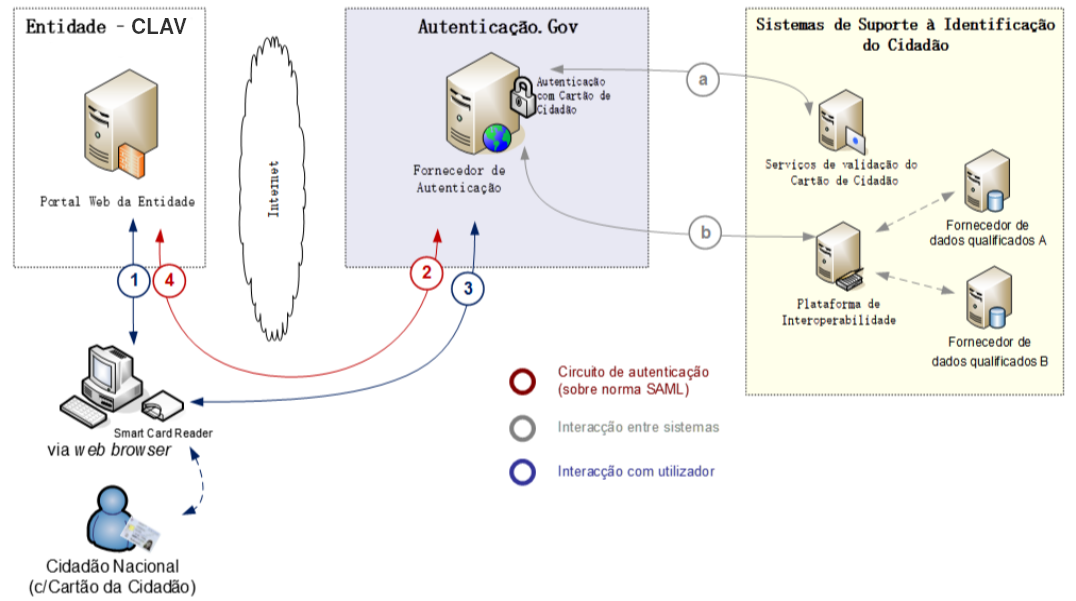
\includegraphics[width=1\textwidth]{img/fluxoauthgov.png}
    \end{center}
    \caption{Fluxo de pedidos entre \acrshort{clav} e o Autenticação.gov de forma a autenticar um utilizador na \acrshort{clav}. Fonte:~\cite{agov}}\label{fig:fluxoauthgov}
\end{figure}

\begin{enumerate}
    \item O utilizador pretende aceder à área privada do portal de uma entidade (do \acrshort{clav}), na qual é necessário que comprove a sua identidade;
    \item O portal da entidade (\acrshort{clav}) delega a autenticação e redireciona o utilizador para o Autenticação.gov, juntamente com um pedido de autenticação assinado digitalmente;
    \item O Autenticação.gov valida o pedido de autenticação recebido e solicita a autenticação do utilizador com recurso ao seu \acrshort{cc} pedindo a inserção do seu \acrshort{pin} de autenticação. Durante este processo, o Autenticação.gov efetua as seguintes operações internas:
    \begin{enumerate}
        \item Valida as credenciais do utilizador com recurso à \acrshort{pki} do \acrshort{cc} via \acrshort{ocsp}
        \item Obtém atributos que sejam solicitados pelo portal da entidade (\acrshort{clav}) junto dos vários fornecedores de atributos qualificados. Esta operação é efetuada via Plataforma de Interoperabilidade. Este processo pode incluir a obtenção de dados da Federação de Identidades ou de outras Entidades.
    \end{enumerate}
    \item A identificação e atributos do utilizador são autenticadas e assinados digitalmente pelo Autenticação.gov, após o que redireciona o utilizador de volta ao portal da entidade original (\acrshort{clav}). Cabe à entidade (\acrshort{clav}) a validação das credenciais do Autenticação.gov e utilização dos atributos do cidadão.
\end{enumerate}

A troca de pedidos entre o \acrshort{clav} e o Autenticação.gov é feita através de \acrshort{saml} 2.0 (com as extensões que a \acrshort{ama} considera obrigatórias). De seguida será feita uma pequena introdução ao \acrshort{saml} 2.0. 

\subsection{\acrshort{saml} 2.0}
O \acrfull{saml} define uma \textit{framework} \textit{standard} em \acrshort{xml}.~\cite{sam2man} Foi aprovado pela \acrshort{oasis} e permite a troca segura de informação de autenticação e autorização entre diferentes entidades. Através do \acrshort{saml} é possível através de uma credencial (\textit{login} de um utilizador) aceder autenticado a um conjunto de \textit{websites}. Esta funcionalidade é conhecida por \acrfull{sso}.

Existem três tipos de papéis em \acrshort{saml}:~\cite{wisaml}
\begin{itemize}[leftmargin=2cm]
    \item Utilizador
    \item \textit{Identity Provider}: Realiza a autenticação de que o utilizador é quem diz ser e envia essa informação ao \textit{Service Provider} junta com as permissões de acesso do utilizador para o serviço
    \item \textit{Service Provider}: Precisa de autenticação do \textit{Identity Provider} para poder dar autorização ao utilizador
\end{itemize}

O documento \acrshort{xml} enviado pelo \textit{Identity Provider} para o \textit{Service Provider} é conhecida por \textit{\acrshort{saml} Assertion}. Existem três tipos de \textit{\acrshort{saml} Assertion}:~\cite{wisaml}
\begin{itemize}[leftmargin=2cm]
    \item \textit{Authentication Assertion}: Prova a identificação de um utilizador e fornece a hora em que o utilizador se autenticou e o método de autenticação usado
    \item \textit{Attribution Assertion}: Envia \textit{\acrshort{saml} attributes} (formato de dados que contém informação acerca do utilizador) para o \textit{Service Provider}
    \item \textit{Authorization Assertion}: Indica se o utilizador está autorizado a usar o serviço ou se o \textit{Identity Provider} recusou o pedido à inserção de uma password errada ou por falta de permissões para usar o serviço
\end{itemize}

No projeto \acrshort{clav} o utilizador final é o utilizador da \acrshort{clav}, o \textit{Identity Provider} é representado pelo Autenticação.gov e o \textit{Service Provider} é representado pela \acrshort{clav}.

%TODO
%\section{exceljs}
    %procurar "semelhantes" para cada um

\section{MongoDB}
~\cite{wdmongo}

%TODO
%\section{mongoose}
%procurar "semelhantes" para cada um

\section{Web Semântica}
~\cite{lsparql}

\subsection{RDF}
~\cite{lsparql}

\subsection{SPARQL}
~\cite{lsparql}

%se calhar referir algumas packages de ligação ao sparql em vez de usar o que criei

\section{GraphDB}
%procurar "semelhantes" para cada um (Neo4j)

\section{Swagger}
%procurar "semelhantes" para cada um

\section{Swagger-UI}

%TODO
%\section{yaml-include}
%procurar "semelhantes" para cada um

%TODO
%\section{swagger-ui-express}
%procurar "semelhantes" para cada um

%TODO
%\section{js-yaml}
%procurar "semelhantes" para cada um

%TODO
%\section{Nginx}
%~\cite{nginxcook}
%procurar "semelhantes" para cada um

%TODO
%\section{Ontologia}
%~\cite{bontology}
%conceito

%TODO
%\section{Docker}
%~\cite{udocker}
%procurar "semelhantes" para cada um

%TODO
%\section{Docker Compose}
%~\cite{udocker}
%procurar "semelhantes" para cada um
